\documentclass[journal]{IEEEtran}
\usepackage{tablefootnote}
% Some Computer Society conferences also require the compsoc mode option,
% but others use the standard conference format.
%
% If IEEEtran.cls has not been installed into the LaTeX system files,
% manually specify the path to it like:
% \documentclass[conference]{../sty/IEEEtran}









% *** GRAPHICS RELATED PACKAGES ***
%
\ifCLASSINFOpdf
\usepackage{graphicx}

\usepackage{booktabs} % lluis added these:
\usepackage{multirow}
\usepackage{siunitx}
  % \usepackage[pdftex]{graphicx}
  % declare the path(s) where your graphic files are
  % \graphicspath{{../pdf/}{../jpeg/}}
  % and their extensions so you won't have to specify these with
  % every instance of \includegraphics
  % \DeclareGraphicsExtensions{.pdf,.jpeg,.png}
\else
  % or other class option (dvipsone, dvipdf, if not using dvips). graphicx
  % will default to the driver specified in the system graphics.cfg if no
  % driver is specified.
  % \usepackage[dvips]{graphicx}
  % declare the path(s) where your graphic files are
  % \graphicspath{{../eps/}}
  % and their extensions so you won't have to specify these with
  % every instance of \includegraphics
  % \DeclareGraphicsExtensions{.eps}
\fi
% graphicx was written by David Carlisle and Sebastian Rahtz. It is
% required if you want graphics, photos, etc. graphicx.sty is already
% installed on most LaTeX systems. The latest version and documentation
% can be obtained at: 
% http://www.ctan.org/pkg/graphicx
% Another good source of documentation is "Using Imported Graphics in
% LaTeX2e" by Keith Reckdahl which can be found at:
% http://www.ctan.org/pkg/epslatex
%
% latex, and pdflatex in dvi mode, support graphics in encapsulated
% postscript (.eps) format. pdflatex in pdf mode supports graphics
% in .pdf, .jpeg, .png and .mps (metapost) formats. Users should ensure
% that all non-photo figures use a vector format (.eps, .pdf, .mps) and
% not a bitmapped formats (.jpeg, .png). The IEEE frowns on bitmapped formats
% which can result in "jaggedy"/blurry rendering of lines and letters as
% well as large increases in file sizes.
%
% You can find documentation about the pdfTeX application at:
% http://www.tug.org/applications/pdftex


\usepackage{scrextend} % mg added this. use the same footnote mark 
\usepackage{gensymb}

% *** MATH PACKAGES ***
%
\usepackage{amsmath}
%\usepackage{breqn}

% *** PSEUDO CODE PACKAGE ***
\usepackage[]{algorithm2e}


\usepackage[hyphens]{url}
% url.sty was written by Donald Arseneau. It provides better support for
% handling and breaking URLs. url.sty is already installed on most LaTeX
% systems. The latest version and documentation can be obtained at:
% http://www.ctan.org/pkg/url
% Basically, \url{my_url_here}.






\begin{document}
%
% paper title
% Titles are generally capitalized except for words such as a, an, and, as,
% at, but, by, for, in, nor, of, on, or, the, to and up, which are usually
% not capitalized unless they are the first or last word of the title.
% Linebreaks \\ can be used within to get better formatting as desired.
% Do not put math or special symbols in the title.
\title{An efficient 3-D sound experience for mobile applications}


% author names and affiliations
% use a multiple column layout for up to three different
% affiliations
\author{\IEEEauthorblockN{Group 3}
\IEEEauthorblockA{
Aalborg University\\
Copenhagen, Denmark\\
}}


% conference papers do not typically use \thanks and this command
% is locked out in conference mode. If really needed, such as for
% the acknowledgment of grants, issue a \IEEEoverridecommandlockouts
% after \documentclass

% for over three affiliations, or if they all won't fit within the width
% of the page, use this alternative format:
% 
%\author{\IEEEauthorblockN{Michael Shell\IEEEauthorrefmark{1},
%Homer Simpson\IEEEauthorrefmark{2},
%James Kirk\IEEEauthorrefmark{3}, 
%Montgomery Scott\IEEEauthorrefmark{3} and
%Eldon Tyrell\IEEEauthorrefmark{4}}
%\IEEEauthorblockA{\IEEEauthorrefmark{1}School of Electrical and Computer Engineering\\
%Georgia Institute of Technology,
%Atlanta, Georgia 30332--0250\\ Email: see http://www.michaelshell.org/contact.html}
%\IEEEauthorblockA{\IEEEauthorrefmark{2}Twentieth Century Fox, Springfield, USA\\
%Email: homer@thesimpsons.com}
%\IEEEauthorblockA{\IEEEauthorrefmark{3}Starfleet Academy, San Francisco, California 96678-2391\\
%Telephone: (800) 555--1212, Fax: (888) 555--1212}
%\IEEEauthorblockA{\IEEEauthorrefmark{4}Tyrell Inc., 123 Replicant Street, Los Angeles, California 90210--4321}}


% *****************************************************************************************************
% *****************************************************************************************************
% added by mg. it is the structure that Stefania suggested use to use
% THIS SHOULD BE THE MAIN STRUCTURE OF THE PAPER
% Here is the structure
% 1) Abstract: a summary of the project and results
% 2) Introduction: Your problem, state of the art
% 3) Implementation: description of your app, the 3D sound features, the sounds,etc….
% 4) Experiment design
% -description of experiment
% -data analysis
% -discussion
% 5) Conclusion 
% -your conclusion
% future work
% -references
% Appendix
% with implementations, etc….all you did which does not fit inside the paper
% *****************************************************************************************************
% *****************************************************************************************************

% use for special paper notices
%\IEEEspecialpapernotice{(Invited Paper)}
% The paper headers

\markboth{3D audio navigation, December~2015}%
{Shell \MakeLowercase{\textit{et al.}}: Bare Demo of IEEEtran.cls for Journals}
% The only time the second header will appear is for the odd numbered pages
% after the title page when using the twoside option.
% 
% *** Note that you probably will NOT want to include the author's ***
% *** name in the headers of peer review papers.                   ***
% You can use \ifCLASSOPTIONpeerreview for conditional compilation here if
% you desire.




% If you want to put a publisher's ID mark on the page you can do it like
% this:
%\IEEEpubid{0000--0000/00\$00.00~\copyright~2012 IEEE}
% Remember, if you use this you must call \IEEEpubidadjcol in the second
% column for its text to clear the IEEEpubid mark.



% use for special paper notices
%\IEEEspecialpapernotice{(Invited Paper)}




% make the title area
\maketitle

% As a general rule, do not put math, special symbols or citations
% in the abstract
\begin{abstract}

%\\ \textit{previous version}\\
%We developed an application for mobile devices that uses an efficient head related transfer function model based on to create 3D soundscapes. The HRTF model is based on a combination of filters and delays provided on theoretical basis by Brown et. al. [1]. The device orientation is used to set the angle between the sound and the user. This model has many possibilities on the limited hardware capabilities of the mobile devices in comparison to HRTF database based models. The prototype will present the user several sounds scattered in a limited area where the user can interact with.

%{\textit{matteo's version...and Andrea's changes :)}}\\
The computational power of mobile devices has highly increased in the last few years and nowadays having a device with Global Positioning System (GPS) and compass sensor has become commonplace. These facilities opens up possibilities to enhance the user experience in daily life. In this paper an application for mobile devices that uses an efficient head related transfer function (HRTF) model to create 3-D soundscapes is presented. In a small experiment the developed 3-D audio engine is compared with a cosine panner model~\cite{AndyFarnell2010} in terms of quality and efficiency of the navigational cues. Although the experiment did not reveal significant differences between the two models a critical observation of this study supports that a more sophisticated 3-D audio engine can increase the user experience in audio navigation.
\end{abstract}


% Note that keywords are not normally used for peerreview papers.
\begin{IEEEkeywords}
Head related transfer function (HRTF), mobile devices, Global Positioning System (GPS), soundscape, Pure Data, OpenFrameworks
\end{IEEEkeywords}



\section{Introduction}
A lot of research on modeling 3-D sound has been done with fairly good results~\cite{begault19943}. The best results can be obtained by those models implementing 3-D sound using personalized head related transfer functions (HRTF), which need tedious measuring of impulse responses for each individual and require large databases ~\cite{SpatialAudio2007, Meshram2014}. Mobile applications as well as multimedia productions are usually aimed at a big number of users, thus implementing HRTFs requiring measurements of the individual user is highly unpractical. Furthermore the convolution needed for using databases with head related impulse responses (HRIR) is an unnecessary heavy technique in terms of computational power and memory, two requirements that are not abundant in mobile devices. Therefore, the aim of this project was to develop a computationally efficient and general HRTF model, yet, keeping the quality of a 3-D sound experience as good as possible. We used the model provided on a theoretical basis in~\cite{Brown1997} by implementing a combination of filters and delays in Pure Data and C. This audio engine was then embedded in a mobile application. Compass and GPS data provided by the mobile device was filtered and then used to compute the apparent direction and distance to the sound source. The purpose of the application was to let the users discover a virtual sound space situated in Copenhagen. Thus, the 3-D audio engine should to satisfy two major requirements:
% tenses in past...?
\begin{enumerate}
    \item It should provide direction cues that are efficient in guiding the user to the position where a specific sound is situated.
    \item It should provide an intuitive way of locating a sound source from a qualitative point of view.
\end{enumerate}

The first aim refers to the speed at which the user can find a sound source receiving only the auditory cues, which optimally would not differ to a great extent of the time needed to navigate to the position of a natural sound source. The 3-D audio engine should yield better or at least as good result as a simple stereophonic panning as some studies already provided evidence of the efficiency of a simple panning to guide the user to a specific location\textbf{ COMMENT:LARS[Here we have to put some citations]\cite{}}. Our second aim was that the model should give a qualitatively more natural and intuitive feeling of the sounds position in the space compared to the panning. While for the panning some level of abstraction as simple as hearing the sound louder from the left meaning that the sound is at the left has to be applied, with the 3-D audio engine we aimed to model a sound coming from a certain direction in a more natural way using a HRTF model which combines direction, distance and externalization cues.

In this paper, first, state of the art research on audio augmented reality will be elaborated to set the theoretical framework. In the second part, the implementation of an efficient and general HRTF model for mobile devices will be presented. Thereafter, to evaluate the implemented model, a comparative study between the 3-D audio engine and a simple stereophonic panning will be presented, and its results based on qualitative and quantitative measures will be discussed. In the last part, a thorough discussion of the results in light of the two demands to the implemented 3-D audio engine will be presented and conclusions will be drawn.

\subsection{State of the art in audio augmented reality}
Recently, the progress in audio technology and computing paved the way for the introduction of completely new types of interactive audio applications~\cite{harma2004}. Advances in mobile technologies have made possible to create audio augmented spaces almost anywhere. For instance, spatial auditory displays that can provide the user with landmarks and are capable to attract the user's attention have been tested and introduced~\cite{alvarez2011}. \emph{COMMENTS:LARS[Do we need this sentence? Because we say nothing about multiple sound sources except for the future works. So maybe we can put it there] ANDREA: I agree with Lars :) ->} Many experiments assessing qualitative and quantitative measures have been designed so far to better understand the way in which people usually perceive multiple simultaneous sources differently placed and to increase the level of immersion in the experience.\\

Theoretically, audio augmented reality has to be distinguished from the traditional concept of a virtual reality audio environment~\cite{harma2004}. In virtual reality, generally participants are abstracted from the natural environment and are surrounded only by a completely synthetic one (acoustic and/or visual). On the opposite, in augmented reality a virtual environment is \emph{superimposed} on a real one. To be more specific, in a mobile audio augmented environment participants are able to interact with the virtual audio mixed with a real visual scene and/or auditory soundscape~\cite{alvarez2011}.\\

\textbf{COMMENT:LARS [We have to reformulate this one once the citation is put in ;)] we wait for Mattia} According to this definition, audio augmented reality (AAR) should be within the boundaries of 1) a perfect augmentation of the listener's auditory environment and is achieved when the listener is unable to predict whether a sound source is part of the real or the virtual audio environment and 2) a set of artificial sounds that are not possible in the real world superimposed and fitted to the visual perceived world like in described in Harma et. al. \cite{harma2004}. Any combination of these two fall within the boundaries of AAR.\\


\subsubsection*{Human sound localization}~\\

The auditory system provides the necessary information to localize sound sources in various dimensions (width, height, depth), process which takes place in the brain \cite{Rumsey2001}.

When a sound event occurs, waves travel in all directions and when  they  reach us,  our  brain  compares  the signals  received  by  the  left  and  right  ears  in order to determine the sound source position.  The signal spectrum reaching both ears is different, since the amplitude and phase information differ~\cite{Rumsey2001}. These binaural cues are  called  \emph{interaural  intensity  difference}  (IID)  and  \emph{interaural time  difference}  (ITD). However, these cues are not enough to localize accurately the source since with this information the listener can not determine if the sound is in front, above or behind. This region where all sounds yield the same ITD and IID is called \textit{cone of confusion}~\cite{SpatialAudio2007}.
This ambiguity can be solved with the information provided by the filter effect caused by the pinna, head, shoulders and torso, which modify the spectrum of the sound that reach the listener's ears. Additionally, other cues as head movements and visual cues  help to reduce these localization ambiguities ~\cite{SpatialAudio2007}.  The sum of all these features are characterized by the head related transfer functions (HTRF) which are not only frequency and direction-dependent but also differ from person to person \cite{Rumsey2001}. That dependency makes therefore hard to generalize the spectral features among individuals. It is well known that using a HTRF from one person in another can significantly impair the  perception due to individual differences in anatomy, but it has also been shown that some people localize better the sounds than others, and their HTRFs are suitable for a large group of listeners \cite{SpatialAudio2007}. Therefore there is some evidence that it is possible to generalize, and it is worth to allow the listener choose their own HRTF set \cite{Tame2012}, although the people localize better with their own HRTFs. 

On the other hand, it is possible to render binaural audio using personalized HRTFs with some methods, as the one presented in \cite{SpatialAudio2007}, which is based on parametric representations of the HRTFs instead of convolution.\\

%don't require a convolution process with the impulse responses.
 
%Thus, having a database with own measured HRTF for each user would be the ideal case. However, because of the large amount of data that the customized HTRFs required to generate externalized virtual sources would entail, and the expensive real-time computation of them every time the sound source moves, this is almost impossible. In addition, due to the limited memory space of the mobile devices, having a database with standard HTRFs would not be the best choice and it is desirable to find a more efficient HTRF model.\\

\subsubsection*{Localization/Lateralization}~\\

In order to have a well binaural reproduction, the features of the HRTFs must be accurately simulated at the listener's ears. Fortunately, the use of headphones facilitates this work since the different signals played to the user's ears can be manipulated separately and individually~\cite{plenge1972}.

However, one of the most critical problem when using headphones is the disability of the listener to hear the sound source placed in the physical space. Instead, it is often perceived inside the head ~\cite{harma2004}, effect which is usually called \emph{lateralization}, or intracranial, or `inside-head-localization` (IHL). On the opposite, the effect of hearing the sound outside the head, according to specific direction and distance, is called \emph{localization} or `outside-head-localization` (OHL)~\cite{plenge1972}. This difference in terminology serves to emphasize the difference between a sound source conveyed directly by headphones and a real source, as underlined by Plenge in~\cite{plenge1972}. It has also been demonstrated that a listener can clearly distinguish when listening through headphones between localized and lateralized sounds sources and that both types can coexist in the listener's experience~\cite{harma2004}.\\


\subsubsection*{Issues in headphones-conveyed sound}~\\

Reproduction of sound through headphones often produces an incorrect localization of virtual sound sources~\cite{harma2004} and many issues could be experienced.\\
\paragraph{Externalization errors}
%Comment Andrea: this sentence is not very clear...can we delete it?Externalization of the sound is related to the perception of auditory distance such that there is a continuum in perceived locations of sources from inside the listener's head to any external position~\cite{hartmann1996}. 
Externalisation is related to the perception of distance between the head and the sound source \cite{Tame2012}. One of the most relevant problems in AAR is the perceived effect of \emph{lateralization}, i.e. the sounds appear to be inside the listener's head. To avoid such effect several techniques can be used. For instance, as expressed in~\cite{harma2004}, the effect of a lateralized sound in headphone listening can be produced using amplitude and delay differences between two headphone signals. The main goal of virtual acoustic synthesis should be to produce sounds that seem \emph{externalized}, that is, outside the listener's head ~\cite{begault2001}. In order to make a sound source externalized and let the user be capable of a correct judgment of the distance of the sound, more sophisticated binaural techniques are needed. In particular, spectrum differences in the HRTF between the two ear signals, play an important role, as also expressed in~\cite{harma2004}. Moreover, acoustic cues such as the amount of reverberation and control of signal level are necessary for a successful auralization of a virtual sound source. Finally, also dynamic cues related to head turning and other movements of either a listener or a sound source should be taken into consideration when dealing with externalization. As described in Harma et. Al.~\cite{harma2004} unnatural changes in the acoustic properties of the virtual sound sources should be avoided, which could be caused by some user intentionally or unintentionally movement.

\paragraph{Localization errors}
Localization error refers to the deviation of the reported position of a sound source from a measured `target` location, i.e. the listener fails in matching the correct location of the sound. Localization errors can be divided in \emph{azimuth} (deviations along the horizontal plane) and \emph{elevation} errors (deviation from eye-level elevation)~\cite{begault2001}. These errors might come from some location accuracy. Determining the accurate position of the user is one of the most important task in an AR system owing to that system always produces output to the used based on his or her location in space~\cite{rozier2000}. That said, any location inaccuracy should be avoided using GPS receiver with high sensitivity and reliability. Here, the implementation design takes a crucial role as noted in~\cite{alvarez2011}.

\paragraph{Reversal errors}
Sometimes called front-back or back-front `confusion`, that error refers to the judgment of a sound source as located on the opposite side of the interaural axis than the target position~\cite{begault2001} due to the cone of confusion. An informal proposal has been made, which tries to help the user in front-back discrimination on the basis of the familiarity of the effects on timbre cues, e.g. unique patterns in \emph{early reflections} depending on the virtual sound location~\cite{begault1992}. Indeed, this has not yet been verified experimentally. (COMMENT - mattia: is it necessary the following sentence?) However in application where the listener can change its angle to the source, the front and back will soon be obvious through the movement of the sound. (MG: insert references for previuos sentences).\\

\subsubsection{Related works}
\emph{Audio Aura} \cite{mynatt1997} was one of the first projects to deal exclusively with audio in augmented reality systems. It basically consisted in providing auditory information to users as they traveled through their workspace. These information was triggered as soon as the subjects entered particular locations in the workspace. The auditory cues used in \emph{Audio Aura} were particularly interesting because most of them were associated to sounds from nature rather then recorded vocal, speech or synthetic sounds. Similar in approach to \emph{Audio Aura} was the \emph{Automated Tour Guide} \cite{bederson1995} COMMENT:LARS[ add something more about that automated tour guide like: ... in which subjecta had to do ...]. In both cases, triggers are readily identifiable, still and rarely changing. The sounds were assigned to pre-determined locations in space and there was no need to determine the precise location of an individual except for knowing when the individual entered the area of interest. COMMENT:LARS[How did they know when to play the sound??? ]\\

A successive work, \emph{Hear\&There} was able to determine the location and head position of the user using the information from GPS and a digital compass~\cite{rozier2000}. A user could listen to these `audio imprints`COMMENT:LARS[is this a direct citation?] by walking into the area that a specific imprint occupied, which then was triggered. The essential premise of  \emph{Hear\&There} was that a physical environment has been augmented with audio. All the sounds and the data were gathered inside that system. Since a `Field Use` has been developed, in which the user wear a hardware portable system, \emph{Hear\&There} has undoubtedly contributed to an improved definition of mobile augmented reality environment. COMMENT:LARS[I am not sure if it contributed to the definition, rather then just falling into the definition?]\\

More recent works in this field use mobile devices to render soundscapes and let the users interact with them. One example is the \emph{In Situ Audio Services} (ISAS) application \cite{aroundMe}, addressed to blind users, which has been a significant reference for the work presented here. ISAS uses the GPS and orientation sensory data of the mobile device to feed an audio engine based on interaural time differences (ITD) and a low pass filter to reduce the back-front confusion.
% 2012

\section{Design, Implementation and Mobile Application}
\subsection{Introduction}
Given the high computational and memory costs that using a spatial audio model based on a traditional HRTF implies, the existing mobile applications employ different approaches to localize the sound. In the development of ISAS,  Blum and Bouchard discarded the usage of the Pure Data Extended object [earplug$\sim$]\footnote{https://puredata.info/downloads/earplug}, which is a real-time binaural filter based on KEMAR impulse measurement, due to its high CPU usage. Instead and as said before, they used simple panning techniques combined with ITD and filtering effects. For this work, [earplug$\sim$] was also considered, but it showed low accuracy. Hence, it was not been tested on a mobile device.

One of the aims of this project was to implement the HRTF model introduced by Brown and Duda in ~\cite{Brown1997} on a mobile application. This model allows an efficient processing of multiple sounds in real time and it has been implemented  in Pure Data and C. A more detailed description of the implementation follows.

Some of the challenges that this implementation has presented are: 1) Does an HRTF model improves the navigation in comparison to a simpler model? 2) How many sounds can be rendered using it?

This project focused on evaluating the improvements that this HRTF model presents in terms of navigation, and for this purpose two mobile applications were developed. The former used the HRTF model, and the latter used a cosine Panner model~\cite{AndyFarnell2010}. This is detailed in the experiment section of this paper.

Finally, Android is the platform that was used to develop the applications and the libpd\footnote{http://libpd.cc/} implementation of Pure Data was used to build the audio engines of these applications.

\subsection{Audio engine}
The audio engine is the core part of the mobile application. As mentioned before, it is based on the HRTF introduced \cite{Brown1997}, which is claimed to be both efficient and of reasonable quality in order to achieve a satisfying user experience and an efficient real time application. The block diagram given in~\cite{Brown1997} and depicted in Figure \ref{fig:workflow} was followed in order to implement it. A general description of the block diagram and an individual of each of the blocks follow. 

\begin{figure}[h!]
  \centering
    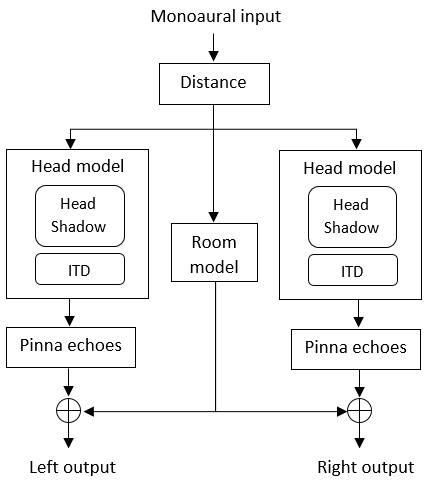
\includegraphics[scale=0.55]{graphics/graphic.jpg}
  \caption{Components of the model provided on a theoretical basis in~\cite{Brown1997}}
  \label{fig:workflow}
\end{figure}

First, a monoaural sound source is processed by a distance model, which will feed in parallel a head model and a room model. The head model stereo output is inputed to a pinna echoes model, whose output is added to the output of the room model to obtain the spatialized version of the sound.

As previously mentioned, to implement the head shadow block of the HRTF model, a Pure Data external called \emph{headShadow} was written in the C programming language. So as to go through this source code development, it was necessary to get the correct difference equation of the head shadow block, which is carefully explained in \emph{The head model} section. It was first implemented in MATLAB and then translated into C code. Except for the Pure Data external, the HRTF model was implemented completely using Pure Data.

\begin{figure}[h!]
  \centering
    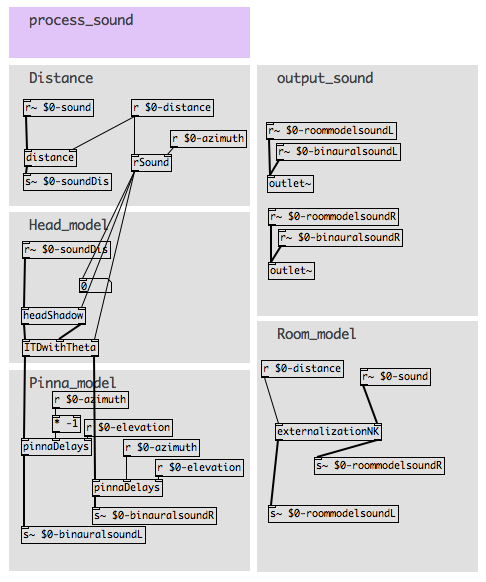
\includegraphics[scale=0.5]{graphics/audioengine.png}
  \caption{The audio engine implemented in Pure Data}
  \label{fig:augioengine}
\end{figure}

\subsubsection{The distance model}~\\
In order to simulate the sound pressure in free field, the inverse distance law was applied. 

\begin{quote}
``Since sound intensity is proportional to the square of sound pressure, the inverse square law (for sound intensity) becomes the inverse distance law (for sound pressure). Therefore, sound pressure is inversely proportional to distance \textit{r}.~\cite{everest2009master}"
\end{quote}

Consequently:
\begin{equation}\label{eq:soundpressure}
P = \frac{k}{r}
\end{equation}

where \textit{P} is the sound pressure, \textit{k} is a constant and \textit{r} is the distance from source.\\

% mg: not sure if we should add the following sentence because there are too many citation from the same passage.
% Hence, for every doubling of distance \textit{r} from the sound source, sound pressure will be halved; i.e. when the distance from the source is doubled, the sound-pressure level decreases by 6 dB~\cite{everest2009master}.

\subsubsection{The head model}~\\
The head model is composed of the Interaural Time Differences (ITD) applied to each channel and the and the head shadow effect.

The difference between the paths from the sound source to each of the two ears and the shadowing effect produced by the head at the far ear lead to a delay and a intensity difference in the sound arriving at the left and right ears.
In order to estimate the time delay, the Woodworth's formulas were applied~\cite{Woodworth}: 

\begin{equation}\label{eq:ITDfront}
ITD = (a/c)[\theta + sin(\theta)]   \; [0 \leq \theta \leq \pi/2]
\end{equation}

\begin{equation}\label{eq:ITDback}
ITD = (a/c)[\pi - \theta + sin(\theta)]  \; [\pi/2 \leq \theta \leq \pi]
\end{equation}

where \textit{a} is the approximated head radius in meters, $\theta$ is the azimuth angle in radians and \textit{c} is the speed of sound in meters over seconds. The time differences of the audio signal reaching the head and the ears are therefore:

\begin{equation}\label{eq:ITDL}
T_{L} (\theta) = \frac{a+a\theta}{c}
\end{equation}

\begin{equation}\label{eq:ITDR}
T_{R} (\theta) = \frac{a-a sin(\theta)}{c}
\end{equation}

where $T_{L}$ and $T_{R}$ are the time delays to reach the left and the right ear, respectively. 

These formulas refer to a source placed in front of the head and on the right, with azimuth $0 \leq \theta \leq \pi/2$. If the source is placed on the left ($- \pi/2 \leq \theta \leq 0$), the expressions are reversed.


% We therefore used the analog filter models provided in \cite{Brown1997} and further specified in \cite{Brown1997}.

% The head shadow filter, implementing the ILD, was given by the following analog transfer function:
The head shadow effect is characterized in the following analog transfer function taken from \cite{Brown1997}:
\begin{equation}\label{eq:analog}
H\left( s,\theta\right) = \frac{\alpha (\theta)s+\beta}{s+\beta},\: where\:\beta = \frac{2c}{a}
\end{equation}


Since it is an analog transfer function, it was derived to a digital version. Therefore, the following transfer function was obtained \footnote{For the derivation of Equation~\ref{eq:filterparam} see appendix A}:
\begin{equation}\label{eq:filterparam}
H\left( z,\theta\right) = \frac{2\alpha (\theta)+T\beta+z^{-1}(-2\alpha(\theta)+T\beta)}{2+T\beta+z^{-1}(-2+T\beta)} = \frac{Y(z)}{X(z)}
\end{equation} 

And, hence, the following difference equation\footnote{For the derivation of Equation~\ref{eq:out} see appendix B}:
\begin{equation}\label{eq:out}
Y[n] =\frac{a_0X[n]+a_1X[n-1]-b_1Y[n-1]}{b_0}
\end{equation} 

where $a_0 = 2\alpha (\theta)+T\beta$ and $a_1 = -2\alpha(\theta)+T\beta$ as well as $b_0 = 2+T\beta$ and $b_1 = -2+T\beta$ are the filter coefficients.\\
% Since we could not use the filter function in Matlab which has as input values the filter coefficientes we had 

%To obtain the difference equation, it was necessary to isolate the output $Y(z)$ in Equation~\ref{eq:filterparam} as well as going from frequency domain to time domain. The result is given in Equation~\ref{eq:out}\footnote{For the derivation of Equation~\ref{eq:out} see appendix B}:
%\begin{equation}\label{eq:out}
%Y[n] =\frac{a_0X[n]+a_1X[n-1]-b_1Y[n-1]}{b_0}
%\end{equation} 

\subsubsection{The pinna model}~\\
High frequency components reaching the listener's ears are affected by the pinna surface, which provides elevation cues and some azimuth information~\cite{Brown1997}. However, in the mobile application the elevation is not considered since all the sound sources are placed in the horizontal plane. 

The pinna model has the following form:

\begin{figure}[h!]
  \centering
    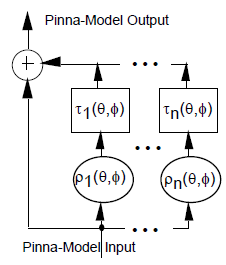
\includegraphics[scale=0.75]{graphics/pinna_part.png}
  \caption{Pinna model. Image taken from~\cite{Brown1997}}
  \label{fig:pinnaModel}
\end{figure}


where the $\rho_{k}$ are the reflection coefficients and the $\tau_{k}$ are the time delays of the \textit{k}th event of a total of \textit{n}. Informal listening tests showed that 5 events were enough to represent the pinna response and that it was convenient to use constant values for the amplitudes $\rho_{k}$,  independent of azimuth, elevation and the subject~\cite{Brown1997}. 

The time delays seem to be properly approximated by the following formula:

\begin{equation}\label{eq:pinna}
\tau_{k}(\theta,\phi) = A_{k}cos(\theta/2)sin(D_{k}(90\degree-\phi)) + B_{k}
\end{equation} 

In this equation, dependent on the azimuth and elevation, the $A_{k}$ is an amplitude, $B_{k}$ an offset and $D_{k}$ is a scaling factor that should be adapted to individual listener. 
In the following table one can see the values for the parameters used in the pinna model. Only one set of values for $D_{k}$ in the application have been used.

\begin{table}[h]
\centering
\caption{Pinna model coefficients}
\label{PinnaModel parameters}
\begin{tabular}{|l|l|l|l|l|}
\hline
k & $\rho$  & $A_{k}$ & $B_{k}$  & $D_{k}$   \\ \hline
1 & 0.5   & 1 & 2  & 1   \\ \hline
2 & -1    & 5 & 4  & 0.5 \\ \hline
3 & 0.5   & 5 & 7  & 0.5 \\ \hline
4 & -0.25 & 5 & 11 & 0.5 \\ \hline
5 & 0.25  & 5 & 13 & 0.5 \\ \hline
\end{tabular}
\end{table}



\subsubsection{The room model}
In ~\cite{Brown1997}, it is implied a very simple room model consisting of only one delay with variable delay time and level according to the distance. An attempt to make a similar model was made by setting the delay time to the difference between the direct path from the object to the listener and a path that bounces on the ground half way between the object and the listener. Finally a more complex model was used due to the poor experienced effect and the large alteration (comb filtering) of the sound quality.

The chosen model is based on the reverb algorithm \textit{rev2~} implemented in Pd. Compared to the original model, the amount of early reflections were reduced and spread more out. Through this, a very large but little reflective room was simulated, with a subtle tail, resembling the characteristics of an outdoor environment. \textbf{COMMENT:Llu�s does not understand the following two sentences, could you write them in another way? and use an alternative to "the 2/d"?} The amount of reverb was diminished according to the distance between the user and the virtual sound source. This happens significantly slower than the $2/d$ of the direct sound, namely $8/(15+d)$. In this way the ratio between the direct and the reflected signal changes even though the total level goes down. This model approximates the test data in ~\cite{begault19943}. The \textit{rev2~} has a direct through signal incorporated, but this was removed in order for an easier control for the dry and wet signal relation.

\textbf{COMMENT: could this be in the section future improvements?} A further improvement could implement variable early reflections delay-times. And separate control over reverb tail and early reflections level.


\subsection{Sensor data retrieval}
The implemented mobile application required two kind of input variables to encode the specific location of the sound source in the real world, namely the distance between the sound source and the user, as well as the direction from which the sound source was coming from. This information could be obtained by accessing the GPS\footnote{GPS is a navigation system which provides location information and most of the mobile devices nowadays include a GPS receiver. As explained in~\cite{noble2009} \textbf{COMMENT:[ask Mattia where to find this reference]} the GPS receiver calculates its position by precisely timing the signals sent by the GPS satellites.} and orientation sensors of the mobile device. 

To access the GPS data \emph{ofxMaps}\footnote{https://github.com/bakercp/ofxMaps} and \emph{ofxGeo}\footnote{https://github.com/bakercp/ofxGeo} addons were used.\footnote{The GPS position on an Android platform requires a listening mechanism, which has been implemented in openFrameworks by calling the \texttt{ofRegisterGPSEvent()} in the \texttt{setup()} method of the source code. In the \texttt{ofApp.h} a method was added in order to handle the updates from the Android OS system calls. It is named \texttt{locationChanged()} and adds an event handler for the dispatched event~\cite{noble2009}. Moreover, the \texttt{startGPS()} method is called at the beginning and \texttt{stopPGS()} should be called when quitting the application to avoid an over consumption of phone battery.} With the GPS position of the user it was possible to estimate the distance between the user and the sound source. This computation was done using the \textit{Haversine} formula\footnote{http://www.movable-type.co.uk/scripts/latlong.html}, which expected as input arguments the GPS location of the user (provided by the GPS data of the phone) and the sound source:

\begin{equation}\label{eq:distancehaversine1}
\begin{split}
  a = {\sin}^{2}(\Delta\varphi / 2) + \cos \varphi _1 + \cos \varphi _2 + \sin^2(\Delta\lambda / 2)
\end{split}
\end{equation}
\begin{equation}\label{eq:distancehaversine2}
\begin{split}
  c = 2 * atan2(\sqrt{a},\sqrt{(1-a)}) 
\end{split}
\end{equation}
\begin{equation}\label{eq:distancehaversine3}
\begin{split}
  d = R * c
\end{split}
\end{equation}
where $\varphi$ is the \emph{latitude}, $\lambda$ is the \emph{longitude}, \emph{R} is earth's radius (mean radius = 6,371 km).

In order to compute the azimuth, which is the angle from which the sound source should appear to come from, first, the orientation of the mobile device to the magnetic north pole was extracted.\footnote{For that, the Android API provides access to the TYPE\_ORIENTATION sensor which, apart from other things, returns the orientation of the mobile device to the magnetic North Pole~\cite{AndroidOrientation}.} 

Having the device's position relative to the magnetic North Pole and the sound location the azimuth could be computed using the following method. First of all, the cartesian plane is taken into account and its origin is defined as the device GPS coordinates. Additionaly, it is assumed that the sound location is in the first quadrant. Therefore the sound orientation on the horizonthal plane must be computed and refered to it as \textit{beta}. In order to compute the angle \textit{beta}, a triangle was defined using the mobile device coordinates, the sound coordinates and an immaginary point coordinates. The point's coordinates were defined as the latitude of the mobile device and the longitude of the sound. Second of all, the length of each side of the triangle was computed using the \textit{Haversine} formula. Using the \textit{asin} function the angle \textit{gamma} can be computed which is then substracted by 90 degree and therefore defining \textit{beta}. To compute the azimuth, \textit{beta} is then substracted by the device's position relative to the magnetic North Pole (see appendix for pseudo-code). 

As a last step before sending the data to the audio engine, simple mean filters were applied to smooth the changes in the raw data. Experimentation showed that a buffer size of 49 samples for the distance and averaging over 7 samples for the azimuth offered a good trade-off between delay of feedback to the users actions, and not having sudden jumps in distance or orientation (see figure \ref{fig:rawvsfiltered}). Additionally, an outlier filter was applied to the raw GPS data. In case there was a jump in the GPS data resulting in a difference of two consecutive distance values of more than 30 meters, that outlier was ignored and the last known GPS location was used.

\begin{figure}[h!]
 \centering		
   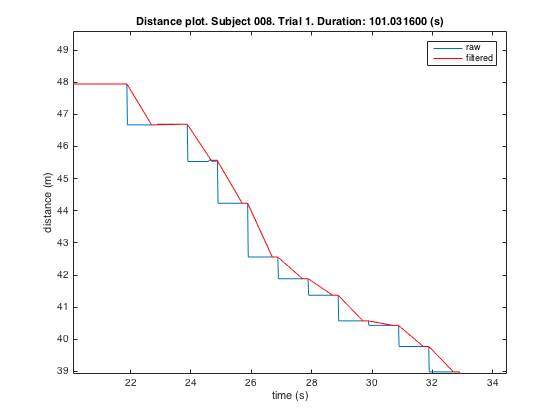
\includegraphics[scale=0.5]{graphics/rawvsfiltered.jpg}		
 \caption{Comparison between raw and averaged distance}		
  \label{fig:rawvsfiltered}		
\end{figure}



% **************************************************************************************************************************
% **************************************************************************************************************************
% Mattia's Version
% Since we are dealing with filtering depending on the sound sources position (e.g. the sound could appear in front of the user as well as behind), it is necessary to take into consideration the user's orientation. That is basically the angle created between the heading of the user and the geographic north pole. Initially, it has been assumed that the user always faced the north, i.e. the angle between the user and the geographic north pole is equal to 0. Discarding the deviation of the user's orientation, it is possible to define the angle between the user and the sound source as the \emph{true bearing \footnote{It is possible refer to it simply as \emph{bearing}.}}. This is, by definition
% \begin{quote}
% {\footnotesize{\textit{the angle measured in degrees in a clockwise direction \footnote{All bearings are measured in a horizontal plane.} from the north line~\cite{} == ask Mattia where did he find this definition == .}}}
% \end{quote}
% Assuming a sound source as a point that radiates in every directions, the bearing of the user from the sound source can be calculated, as shown in (add figure)
% {\footnotesize{\textit{Ask Mattia which figure to add}}}.
% The bearing could be accessed via the \emph{ofxGeo} addon, which contains a specific method called \emph{GeoUtils::bearingHaversine} that uses the \textit{`haversine'} formula:

% \begin{equation*}\label{eq:haversine}
% \begin{split}
%   \theta = & atan2(sin (\delta \gamma)cos(\varphi_2)) cos(\phi_1)sin(\varphi_2)\\
%   &-sin(\varphi_1)cos(\varphi_2)cos(\delta \gamma)) \\
% \end{split}
% \end{equation*}
% where $\varphi$ is the \emph{latitude}, $\delta$ is the \emph{longitude}.
% Once the bearing is determined, it can be assumed that the angle between the heading of the user and the sound source should be the sum of the bearing and the direction the user is facing. Doing so, using a compass it can be retrieved. In order to access the compass orientation a specific addon has been implemented which accesses the `SENSOR TYPE ORIENTATION' provided by the Android API. Having this information four cases has to be differentiated: 
% \\
% {\footnotesize{(some images and explanation about how we calculated the angle between our heading orientation and the sound.)}}
% \\
% In order to smooth the sensor data (especially for the orientation) we filtered the sensory information by computing the median of a chunk of mediansize instances of the sensor output. 
% **************************************************************************************************************************
% **************************************************************************************************************************


\subsection{User interface}
The user interface was designed for the purpose of running the tests mentioned in the introduction. There was one button to start the training trials, and a second one to start the testing trials. 

Since the interface was built only for testing purposes and the listener didn't need to interact with it, the interface was not developed in a user-friendly way (see figure 5). The user interface has not yet been specifically designed for the user.

\begin{figure}[h!]
 \centering   
   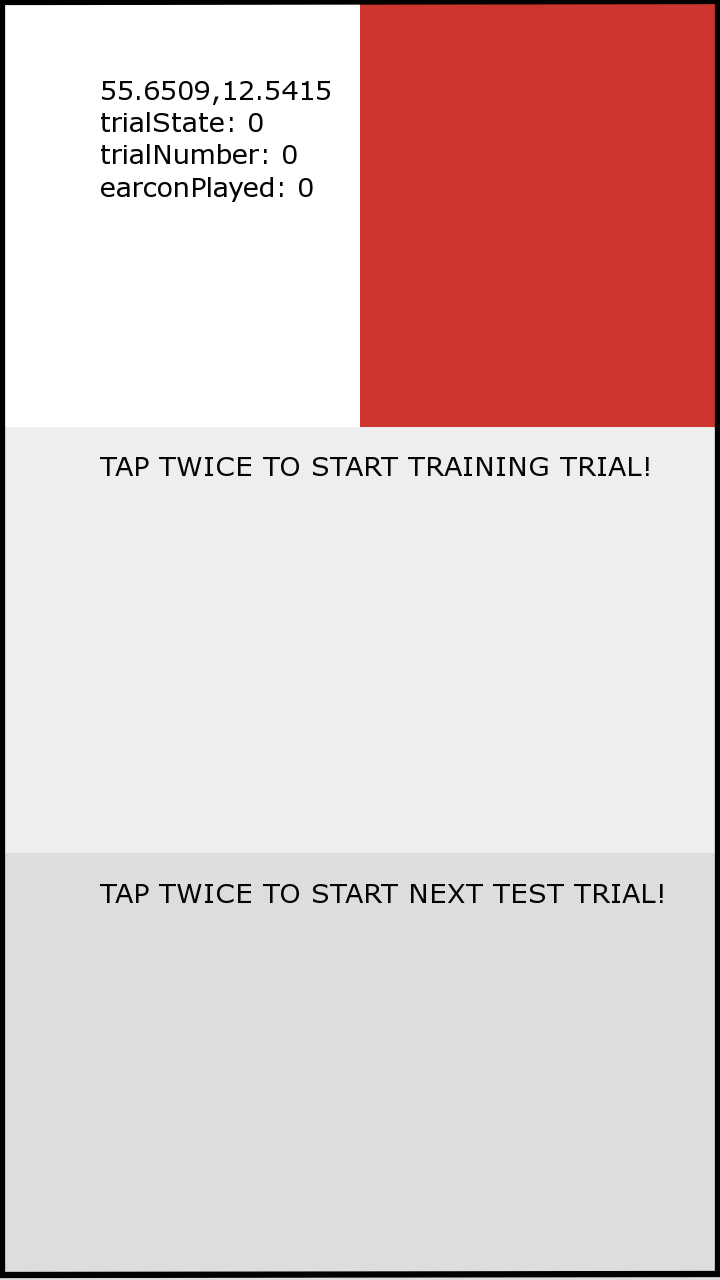
\includegraphics[scale=0.2]{graphics/GUI.png}    
 \caption{Application GUI used for the experiment.}   
  \label{fig:gui}   
\end{figure}

%%%%%%%%%%%%%%%%%%%%%%%%%%%%%%%%%%%%%%%%%%%%%%%%%%%%%%%%%%%%%%%%%%%%%%%%%%%%%%%%%%%%%%%%%%%%%%%%%%%%%
%%%%%%%%%%%%%%%%%%%%%%%%%%%%%%%%%%%%%%%%%%%%%%%%%%%%%%%%%%%%%%%%%%%%%%%%%%%%%%%%%%%%%%%%%%%%%%%%%%%%%
\section{The experiment}
One of the aims of our experiment was to investigate how fast users were able to locate and navigate to a single sound source using our 3-D audio engine compared to a cosine panner based on~\cite{AndyFarnell2010} and 2/d distance calculation which served as a baseline performance. Therefore the time needed from the beginning of a trial until the sound source was found was measured. 

Additionally we assessed a qualitative analysis of how intuitive it was for subjects to locate the sound as well as investigating whether the sound seemed to be embedded in the real scenery. These results were again compared to the cosine panner model~\cite{AndyFarnell2010}. The data was obtained with a 10 point likertscale questionnaire going from ''don't agree at all'' to ''completely agree''.

Results showed no statistically significant results between both models, neither for the quantitative nor qualitative analyses.
%%%%%%%%%%%%%%%%%%%%%%%%%%%%%%%%%%%%%%%%%%%%%%%%%%%%%%%%%%%%%%%%%%%%%%%%%%%%%%%%%%%%%%%%%%%%%%%%%%%%%
%%%%%%%%%%%%%%%%%%%%%%%%%%%%%%%%%%%%%%%%%%%%%%%%%%%%%%%%%%%%%%%%%%%%%%%%%%%%%%%%%%%%%%%%%%%%%%%%%%%%%
\subsection{Materials and methods}
\subsubsection{Participants}
Qualitative data were collected from 11 participants (3 women and 8 men; mean age: 25, ranging from 22 to 30 years). For the quantitative data 6 more participants were measured summing up to in total 17 participants (4 women and 13 men; mean age: 25, ranging from 22 to 30 years). All participants were students coming from different backgrounds.\footnote{However, 14 subjects were master students in Sound and Music Computing at Aalborg University Copenhagen.} Six students were already familiar with 3-D audio sound and four of them had experience in audio navigation before conduction of the experiment. The other participants were naive. All participants reported normal or corrected to normal vision and no hearing deficits. Participants received no form of compensation other than gratitude. 

\subsubsection{Apparatus and stimuli}
The experiment took place in a free field (grass) in "Valby Parken" in Copenhagen, Denmark (Coordinates: 55$^\circ$38'22.3"N, 12$^\circ$31'27.4"E). The mobile device used was a Motorolla Moto G running with Android version 5.0.2. The device was connected to Sony MDR ZX600 stereo headphones. Only one person at a time was tested. 

\begin{figure}[h!]
 \centering		
   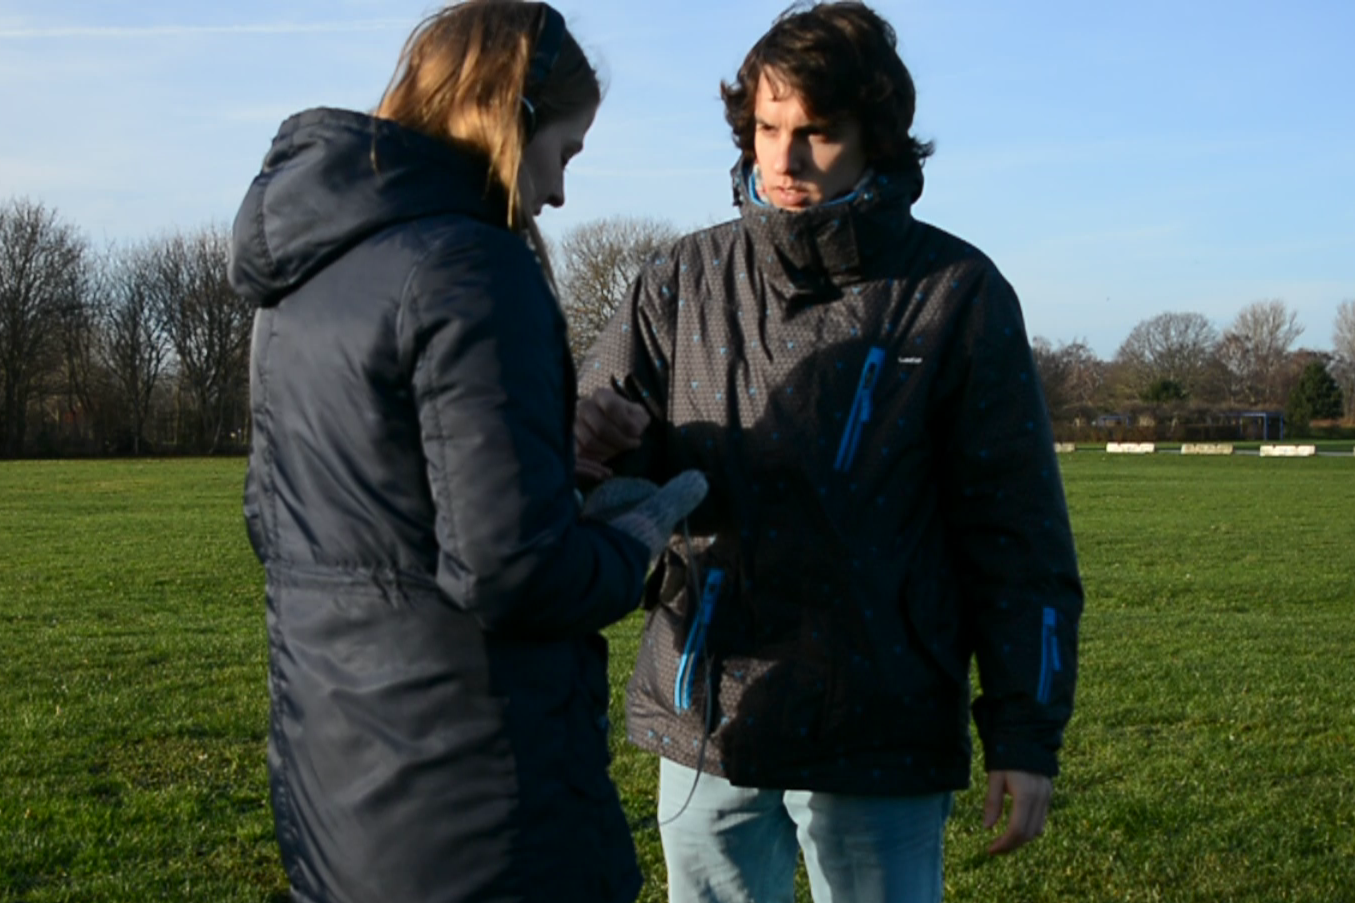
\includegraphics[scale=0.18]{graphics/experiment_AYL}		
 \caption{Testing the application in Valby Parken, Copenhagen}		
  \label{fig:testing}		
\end{figure}

To create the auditory stimulus, digital vocal recordings of a male voice (age: 38) were collected using a AudioTechnica AT4040 condenser microphone and Apogee Duet II� digital audio interface. Recordings were done with 24 bits of resolution for amplitude at a sampling rate of 44100  kHz. Auditory stimuli have been compressed and equalized using a Maag Eq4 parametric equalizer, Teletronik LA-2A and Vertigo VSC-2 Quad Discrete Compressor plugins. They finally have been normalized in peak amplitude using the Izotope Ozone Maximizer (settings: IRC III algorithm, threshold: -7.0 dB, ceiling: -0.2 dB) so that at the minimal distance to the sound source (7 meter) using the maximal level of volume on the mobile device, the sound level of each sound source was at -4.5 dB SPL (see appendix for stimulus content). 

\subsubsection{Design}
The experiment comprised one within subject factor at 2 levels (sound engine). The two levels of the sound engine were our 3-D audio engine (3-D) and a cosine panner~\cite{AndyFarnell2010} and distance amplitude modulation (panning).

The starting point was fixed and the distance of the sound source from that point was always 48 meters.\footnote{However, because of poor GPS accuracy, the location of the sound source was calculated with the momentary GPS coordinates provided by the phone sensor instead of the actual fixed position in the free field. This ensured that the initial distance to the sound source was always the same.} The sound could appear at any angle from the starting point.

For all trials the same soundfile was played. Each participant performed a total of 6 trials meaning 3 trials in each of the two conditions. Participants were encouraged to take a short break whenever they felt fatigued.

\subsubsection{Procedure}
The position (angle from the starting point) of the sound sources in the different trials were completely randomized within and between subjects independently from the sound engine. This ensured that participants could not predict the location of the sound in the next trial. The order of trials with the one or the other sound engine was not randomized within subjects. Nevertheless, half of the participants started the experiment with the 3-D audio engine while the other half started with the audio panning sound engine to counterbalance for effects related to training. After each block of trials (one block were 3 trials with one of the sound engines) participants had to fill out the qualitative questionnaire.

Each trial was initiated by the experimenter with a button press after which the sound source was played. No visual feedback about the location of the sound source or the already passed time to locate it was given. For localization, subjects had to rely solely on the auditory cues given via the headphones. /footnote{Admittedly participants could have used the position of the starting point as some kind of fix point. However, participants did know nothing about the possible distances of the sound source. Additionally, questions after the experiment about applied strategies did not reveal that participants used visual cues for localizing the sound source.} As soon as the participants reached a radius of 7 meter around the sound source, an earcon was played indicating the success of the localization. The participants went back to the initial starting point and the next trial was started.

Before the experiment, participants were familiarized with the target sound as well as the earcons that were played when having reached the location of the virtual sound source. Additionally, all participants performed at least two practice trials with the sound engine they were tested with first before the actual measurements with that sound engine began. The location in the practice trials were fixed at the same positions for all participants to allow us to guide the subject when they got lost. 

Participants were instructed to find the sound source as fast as possible. No information about the possible locations (distances and angles) was given to the subjects. Trials which lasted longer than 5 minutes were aborted and labeled as "not found". 

\subsubsection{Analyses}
For the quantitative analysis 26 trials were excluded because either analyses of GPS data for those trials revealed very poor precision (sudden jumps or no changes in the GPS signal for a period of time) or the orientation sensor got stuck which either increased the time needed to find the sound source to a great extent or made it even impossible for the subjects to locate the sound source within 5 minutes. One subject had to be discarded completely from the analyses because there was no single trial with reliable GPS for the panning engine. The other 16 subjects performed at least one trial in each condition. The remaining trials to be analyzed summed up to 41 trials in the 3-D condition and 42 trials in the panning condition.

For the qualitative analysis the questionaires from 11 participants were evaluated using parametric as well as non-parametric methods as there are arguments in favor \cite{Norman2010, Carifio2007} and against \cite{Kuzon1996} treating likert-scale data as ordinal and/or interval data. 

The threshold chosen to correctly reject the null-hypothesis was always 5\% ($\alpha$ = .05).
%%%%%%%%%%%%%%%%%%%%%%%%%%%%%%%%%%%%%%%%%%%%%%%%%%%%%%%%%%%%%%%%%%%%%%%%%%%%%%%%%%%%%%%%%%%%%%%%%%%%%
%%%%%%%%%%%%%%%%%%%%%%%%%%%%%%%%%%%%%%%%%%%%%%%%%%%%%%%%%%%%%%%%%%%%%%%%%%%%%%%%%%%%%%%%%%%%%%%%%%%%%

\subsection{Results}
\subsubsection{Quantitative}
On average subjects needed 104.6 seconds (SD = 44.8) to find the sounds for the 3-D conditions and 109.8 seconds (SD = 44.1) for the panning condition. 

We computed a paired samples t-test to compare the results for both sound engines which revealed no significant difference between the means for both sound engines (t(15) =-.48, p =.64). However, checking whether our data is normally distributed using the Shapiro-Wilk test showed that for the 3-D data the assumption of normality was violated (Z=.81, p = .004) and close to significance in the panning condition (Z=.89, p =.054). Therefore, we additionally computed the non-parametric Wilcoxon signed rank test which does not assume normal distributed data. Nevertheless, we could not find a significant difference in scores for time needed to find the sound source between both conditions (median: 3-D=85.3, panning=95.9; Z=-.83, p = 0.41 ). 

\subsubsection{Qualitative}~\\
The Shapiro-Wilk test showed that the data was normally distributed both for the 3D model (Z = 0.933, p = 0.44) and the Panning model (Z = 0.95, p = 0.67). 

%Statistical tests applied to each question of the questionnaire do not show significant difference between both sound engines either.
Evaluation of the questionnaires, Table \ref{table:questionnairetable}, showed that the mean and median values for questions 1, 2, 3 and 4 for the 3D model were only numerically different from the panning. Neither the paired samples t-test nor the Wilcoxon signed rank test or the sign test showed significant results comparing the two conditions (3-D vs. panning). However, performing a one sample t-test on means of the four questions for each model comparing it with a neutral response (5.5) showed that users rated the connection between their position and what was presented via the headphones better than neutral for the 3-D sound engine (t(10) = 4.32, p =.002; Z =2.74 , p = .006) but not for the panning (t(10) = 1.07, p = .31; Z = .90, p=.367). For all other questions there were no significant differences.\footnote{It is worth noting that choosing mean and median as 5 instead of 5.5, showed that also for question two, a one sample t-test and the wilcoxon signed rank test were significant for the 3-D (t(10) = 2.52 , p = .03 ; Z = 2.19, p =.028) but not for the panning sound engine (t(10) = 1.19, p = .26 ; Z = 1.2, p =.23).}

\begin{table}[h]
\scalebox{0.85}{

 \begin{tabular}{llllllll}

    \toprule
    \multirow{2}{*}{Question} &
      \multicolumn{2}{c}{Mean (s)} &
      \multicolumn{2}{c}{Std (s)} &
      \multicolumn{2}{c}{Median (s)} \\
& {3D model} & {Panning} & {3D model} & {Panning} & {3D model} & {Panning}\\
      \midrule

1    & 6.36    & 5.91    & 1.75    & 1.70    & 6    & 6    \\
2    & 6.91    & 5.82    & 2.51    & 2.27    & 8    & 6    \\
3    & 7.09    & 6.00    & 1.22    & 1.55    & 7    & 6    \\
4\tablefootnote{It should be noted that for this question lower values represent higher quality of a 3-D sound because of the direction of the question.}    & 6.64    & 6.09    & 2.58    & 1.97    & 7    & 5    \\
5    & 6.09    & 6.55    & 2.21    & 2.54    & 7    & 7    \\


    \bottomrule\\
  \end{tabular}\\
  }
  \caption{Questionnaire results}
  \label{table:questionnairetable}
\end{table}

Summing the results for the first four questions to form an overall category of quality of the two sound engines lead to the mean and median values depicted in Table \ref{table:overallquestionaire}. Again, the difference between both sound engines were only numerically visible since performing a paired samples t-test and a Wilcoxon signed rank test showed no significant results  (t(10) = 1.05, p = 0.32; Z = -1.07, p = .283). Furthermore, running a one sample t-test and wilcoxon signed rank test to compare the results of both sound engines to a mean (5.5) that represents being neutral towards a question showed no significant results for both conditions (HRTF: t(10) = 1.54, p = .154; Z = 1.54, p = .13; Panning: t(10) = -.22, p =.829; Z = -0.5, p = .96). However, summing only the first three questions, showed that the 3-D model ratings were significantly higher than the neutral mean (5.5) (t(10) = 2.83, p = .018; Z = 2.09, p = .036) which was not the case for the panning condition (t(10) = .86, p = .41; Z = 0.76, p = .447).

%\begin{verbatim}
%---- Shapiro-Wilk test 3D model ----
%h1 = 0,  p1 = 0.4444,  w1 = 0.9332

% SWstatistic - The test statistic (non normalized).
%
%   pValue - is the p-value, or the probability of observing the given
%     result by chance given that the null hypothesis is true. Small values
%     of pValue cast doubt on the validity of the null hypothesis.
%
% The null-hypothesis of this test is that the population is normally distributed
%     H = 0 => Do not reject the null hypothesis at significance level ALPHA.
%     H = 1 => Reject the null hypothesis at significance level ALPHA.

%
%---- Shapiro-Wilk test panning ----
%h2 = 0,  p2 = 0.6878,  w2 = 0.9534
%
%---- perform paired samples t-test ----
%ht_test = 0
%pt_test = 0.3199
%ci = [-2.3598 6.5417]
%
%statst_test = 
%    tstat: 1.0468
%       df: 10
%       sd: 6.6250
%
%---- perform Wilcoxen-signed rank test ----
%p = 0.3223
%h = 0
%stats = signedrank: 38
%\end{verbatim}


\begin{table}[h]
\scalebox{0.85}{
 \begin{tabular}{llllllll}

    \toprule
    \multirow{2}{*}{Question} &
      \multicolumn{2}{c}{Mean (s)} &
      \multicolumn{2}{c}{Std (s)} &
      \multicolumn{2}{c}{Median (s)} \\
%& {model 1} & {model 2} & {model 1} & {model 2} & {model 1} & {model 2}\\
& {3D model} & {Panning} & {3D model} & {Panning} & {3D model} & {Panning}\\
      \midrule

1 - 3      & 6.79  & 5.91  & 1.51    & 1.58    & 7.33  & 5.67\\
1 - 4      & 5.93  & 5.41  & 0.93    & 1.36    & 6  & 5.25\\

    \bottomrule\\
  \end{tabular}\\
  
  }
  \caption{Overall results}
\label{table:overallquestionaire}
\end{table}

\section{Discussion}
The results show that both sound engines did not differ in terms of performance. Although numerically subjects were slightly faster to locate the sound source when using the HRTF audio engine, this difference could not be verified statistically. This comfirms that the 3-D audio engine at least partly fulfilled the aims, namely perfoming at least as good as a simple panning. It is also possible that our sample size was so small that the difference in performance would have had to be bigger to show significant results. As noted by several methodologists Type II errors have a high probability to occur for low sample sizes \cite{DeWinter2013}. On top of the small sample size, an unreliable GPS source (different number of GPS satellites fixes for each experiment, with mean of fixes: 11 ranging from 5 to 12) and different weather conditions (subjects complained about wind noises interfering with the auditory display of the soundsource) could have been responsible for the large variance in the data and thus reducing the power of our statistical test \cite{McClelland2000}.

As for the qualitative results looking at the histograms of each questions shows that the differences between the ratings of each participants varied to a great extent. \textbf{COMMENT:Lars[Here we can discuss a little more the results of the hist? subjective?]}. Nevertheless, no statistical differences in user ratings between both audio engines could be found. An explanation for why the 3-D audio engine was not rated better than the panning might have been the choice of a unnatural high reverberation level for a free field in the HRTF audio engine. This is inspired by the fact that a lot of participants had background knowledge in acoustics and therefore made more predictions about a proper reverberation level for a free field. Some subjects even reported the reverberation to be the reason for low ratings of the question regarding whether the sound source was perceived to be embedded in the real scenery. This negative effect on the ratings might have nullified the difference between panning and HRTF in terms of perceiving the sound moving around and not inside the head.

Participants might have had a great top-down expectation of hearing the sounds coming from the headphones rather than being externalized meaning coming from a specific location in the real world. This might have negatively affected the experience of an externalized sound especially considering the lack of a visual representation of the soundsource. 

Nevertheless, it should be noticed that the ratings of the first three questions about the quality of the audio engine taken together (as well as the third question alone which was asking about whether subjects felt the sound to come from outside of their head) were significantly higher than a neutral response for the HRTF but not for the Panning. Figure \ref{fig:histqq13} shows the ratings for the first to third questions taken together, see the appendix \textbf{WHICH ONE?} to see the responses to each questionnaire question. At a first glance this might seem contradictory and has to be considered with caution since panning and HRTF ratings were not significantly different from each other. However, the finding that the HRTF was rated higher than the mean while panning was not could be interpreted as an indication of the superiority in quality of the HRTF over the panning audio engine, especially in rendering the perception of a connection between the users position and the feedback given via the headphones. 

\begin{figure}[h!]
  \centering
    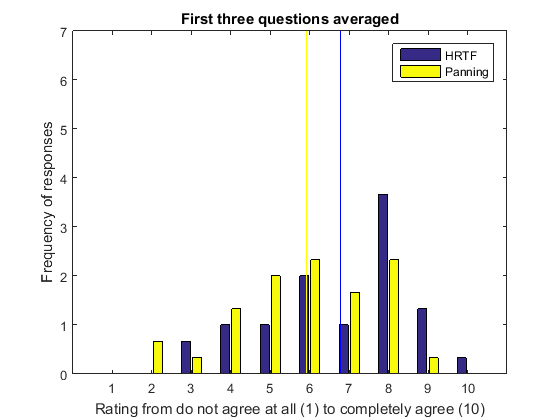
\includegraphics[scale=0.7]{graphics/qq13.png}
   \caption{Distribution of answers for the first three questions}
  \label{fig:histqq13}
\end{figure}

Although, GPS data was filtered the mapping from the actions of the participant to what was registered by the mobile device and given as input to the audio engine might not have been accurate enough for a convenient experience disregarding the audio engine used. Following this logic, even a perfect 3-D audio engine could not have resulted in higher ratings for questions about easyness and intuitiveness to locate the soundsource.

Another issue that should be addressed is the adequacy of the questionnaire used in this experiment. In the present experiment a 10-point likertscale instead of  a 5- or 7- point likertscale was used to achieve a more fine grained rating (higher precision). Since we only had few questions, having so many answer possibilities should not have fatigued the subject too much so that accuracy of the responses should not have suffered due to too many answer possibilities. Though, it has to be noted that subjects were outside when filling out the questionnaire which due to cold temperatures might have driven the subjects to respond in a fast pace leading to less accurate responses. Also the fact that ratings of most of the questions were not significantly different from the mean of the scale itself (indicating being neutral towards the posed question) provides some evidence that subjects were either actually indifferent to the posed questions or had difficulties of knowing which number corresponds to which degree of agreement to the stated question. Additionally, it has been reported that 10-point likert scales produce significantly lower mean values than 5- or 7-point likertscales \cite{Dawes2012}. The just mentioned issues might sum up suggesting that it is rather the method used to assess the qualitative data than the quality of the sound engines themselves that lead to the qualitative results. 

In light of all these considerations the attention should not be drawn away from the fact that the 3-D audio engine is far from being perfect. More thorough evaluation of reverberation levels and distance models can be considered to improve the user experience. Additionally more sophisticated and accurate sensors to track the position of the user relative to the virtual soundsource could enhance the responsiveness of the audio engine. Thereby attention should be payed to the tradeoff between the quality and accuracy of the audio engine itself and the sensors i.e. which level of accuracy of the sensors is needed to meet up with the accuracy of the 3-D audio engine. 
 
\subsection{Future improvements}
Undoubtedly, much refinement and improvement should be made to improve both the quality and the performance of our application. As a prototype, we concentrated mainly on the core, that is to say the programming and sound processing aspects. However, we are conscious that developing a clear and compact GUI is as much important in terms of accessibility to users. In this section several possible improvements will be given. \\
%Multiple sounds
First of all, using multiple sound sources could allow for more interesting and immersive environments. We all are familiar to surroundings made of several items, whose combinations are almost endless. Let's take a crowded place as example. In such similar situation, the user would be given a bunch of different sounds placed in different locations. This is also a crucial point in developing applications such as \emph{Events in the City} and \emph{Audio Tour Guide}. \\
%add front/back discrimination
As said in previous sections, in some experimental situation listeners could make \emph{front-back} discrimination errors. Literature has already dealt with it and has provided numerous suggestions to solve that problem, as depicted in~\cite{blum2012}and~\cite{wightman1999}.\\
%adaptive reverb (maybe a little discussion about pro-cons of convolution)
Use and choice of the right reverb is another crucial point. Even though its choice could be mostly affected by ease of implementation and computational cost, we would aim for an adaptive one, which could be capable of give back a more realistic environment model. Indeed, the choice of a convolution reverb would be the most appropriate since any kind of space could be precisely modelled using its frequency response. On the other hand, it has a huge computational cost, which maybe not all mobile devices couldn't afford. That said, an alternative model of this application should be thought, which all the computing part is shifted on a specific machine. Doing so, the mobile application could be fed directly on externalized sounds.\\
%GUI development and code refinement
Finally, an improvement in graphics is encouraged in to let the application be more appealing and \emph{user-friendly} as well as a code refinement operation to eliminate any superfluous tasks, let all the application be lighter and take advantage of the new technologies structure introducing multithreading.

% discussion
%quantitative:
%- prediction: with more trials maybe there is a learning curve, but not many trials. -> compare mean of subjects to superusers. testing from training could be promising.
%70 s for superusers
%112 for untrained users
%
%- on top of small sample size, and an unreliable gps source (different number of gps satellites fixes, mean of fixes: 11) and also the different weather conditions add up to the large variance and thus the threshold of significance difference between models.
%- 
%- 
%
%qualitative:
%- there is an expectation to hear the sounds from the device. When we hear sounds from an object in the real world, there is an expectation that the sound is coming from there.
%- reverb should also be carefully tested depending on the location of the experiment.
%- we did not achieve a significant externalization factor with the hrtf. future works: improve externalization, so this might help the hrtf






%%%%%%%%%%%%%%%%%%%%%%%%%%%%%%%%%%%%%%%%%%%%%%%%%%%%%%%%%%%%%%%%%%%%%%%%%%%%%%%%%%%%%%%%%%%%%%%%%%%%%
%%%%%%%%%%%%%%%%%%%%%%%%%%%%%%%%%%%%%%%%%%%%%%%%%%%%%%%%%%%%%%%%%%%%%%%%%%%%%%%%%%%%%%%%%%%%%%%%%%%%%

\section{Conclusion}
%add to conclusion:
%that the prototype with multiple sounds is created but further optimization of the code should be necessary to test it given that the sound sources were distorted.
%


% conference papers do not normally have an appendix
%Given that, it could be interesting to replicate the experiment using an external sound source, i.e. a loudspeaker, and compare the trials in which we play from the loudspeaker or headphone
% virtual reality??


% use section* for acknowledgment
\section*{Acknowledgments}






% \begin{thebibliography}{4}

% \bibitem{Brown1997}
% C. Phillip Brown and Richard O. Duda, \textit{An efficient HRTF model for 3-D sound}. Proceedings of the IEEE Workshop on Applications of Signal Processing to Audio and Acoustics. New York: IEEE. 1997

% \bibitem{HowTo}Johannes M. Zmoelnig, \textit{HOWTO write an External for puredata}.\\\texttt{ http://
% pdstatic.iem.at/externals-HOWTO/}, 2010.

% \bibitem{Woodworth}Neil L. Aaronson and William M. Hartmann, \textit{Testing, correcting, and extending the Woodworth model
% for interaural time difference}. Acoustical Society of America, 2014.

% \bibitem{AnalysingLop} P.M. Delgado. \textit{First steps on Pure Data’s approach to real time audio processing. Compiling externals. Analysing lop~}. https://pmdelgado.wordpress.com/2015/09/17/first-steps-on-pure-datas-approach-to-real-time-audio-processing-compiling-externals-analysing-lop/



% \end{thebibliography}


% trigger a \newpage just before the given reference
% number - used to balance the columns on the last page
% adjust value as needed - may need to be readjusted if
% the document is modified later
%\IEEEtriggeratref{8}
% The "triggered" command can be changed if desired:
%\IEEEtriggercmd{\enlargethispage{-5in}}

% references section

% can use a bibliography generated by BibTeX as a .bbl file
% BibTeX documentation can be easily obtained at:
% http://mirror.ctan.org/biblio/bibtex/contrib/doc/
% The IEEEtran BibTeX style support page is at:
% http://www.michaelshell.org/tex/ieeetran/bibtex/
%\bibliographystyle{IEEEtran}
% argument is your BibTeX string definitions and bibliography database(s)
%\bibliography{IEEEabrv,../bib/paper}
%
% <OR> manually copy in the resultant .bbl file
% set second argument of \begin to the number of references
% (used to reserve space for the reference number labels box)
%\begin{thebibliography}{1}
%
%\bibitem{IEEEhowto:kopka}
%H.~Kopka and P.~W. Daly, \emph{A Guide to \LaTeX}, 3rd~ed.\hskip 1em plus
%  0.5em minus 0.4em\relax Harlow, England: Addison-Wesley, 1999.
%
%\end{thebibliography}


\pagebreak
%\listoffigures
%\listoftables
%\pagebreak
\begin{appendices}
\section{Derivations}


The analog transfer function has to be derived to the digital version by applying a bilinear transform:

\begin{equation}\label{eq:bilin}
s = \frac{2}{T} \frac{z-1}{z+1},\: where\:T\:is\:the\:sampling\:interval\:in\:seconds
\end{equation}


Applying the substitution in equation~\ref{eq:bilin} to equation~\ref{eq:analog}, following filter function in the digital domain is obtained:
\begin{equation}\label{eq:filter}
H\left( z,\theta\right) = \frac{\alpha (\theta)(\frac{2}{T} \frac{z-1}{z+1})+\beta}{(\frac{2}{T} \frac{z-1}{z+1})+\beta}
\end{equation}

The derivations followed to get equation ~\ref{eq:filterparam} can be seen as follows

\begin{equation*}\label{eq:DerivationFilterCoeff}
\begin{split}
H\left( z,\theta\right) &=\frac{\alpha (\theta)(\frac{2}{T} \frac{z-1}{z+1})+\beta}{(\frac{2}{T} \frac{z-1}{z+1})+\beta}\\
                                   &= \frac{\frac{2\alpha (\theta)(z-1)}{T(z+1)}+\frac{T\beta(z+1)}{T(z+1)}}{\frac{2(z-1)}{T(z+1)}+\frac{T\beta(z+1)}{T(z+1)}}\\  
			   &=\frac{\frac{2\alpha (\theta)(z-1)+T\beta(z+1)}{T(z+1)}}{\frac{2(z-1)+T\beta(z+1)}{T(z+1)}}\\
			  &=\frac{2\alpha (\theta)(z-1)+T\beta(z+1)}{2(z-1)+T\beta(z+1)}\\
			 &=\frac{z2\alpha (\theta)(1-z^{-1})+zT\beta(1+z^{-1})}{z2(1-z^{-1})+zT\beta(1+z^{-1})}\\
			&=\frac{2\alpha (\theta)(1-z^{-1})+T\beta(1+z^{-1})}{2(1-z^{-1})+T\beta(1+z^{-1})}\\
			&=\frac{2\alpha (\theta)-2\alpha (\theta)z^{-1}+T\beta+T\beta z^{-1}}{2-2z^{-1}+T\beta+T\beta z^{-1}}\\
			&=\frac{(2\alpha (\theta)+T\beta)-(2\alpha (\theta)+T\beta)z^{-1}}{(2+T\beta)-(2+T\beta)z^{-1}}\\
			&=\frac{(2\alpha (\theta)+T\beta)+(-2\alpha (\theta)+T\beta)z^{-1}}{(2+T\beta)+(-2+T\beta)z^{-1}}\\
\end{split}
\end{equation*} 



\begin{equation*}\label{eq:DerivationC++}
\begin{split}
H(z, \theta) &= \frac{Y(z)}{X(z)} = \frac{a_0+a_1z^{-1}}{b_0+b_1z^{-1}}\\
&\iff Y(z)(b_0+b_1z^{-1}) = X(z)(a_0+a_1z^{-1})\\
&\iff Y(z)b_0+b_1Y(z)z^{-1} = a_0X(z)+a_1X(z)z^{-1}\\
&\iff Y(z) = \frac{a_0X(z)+a_1X(z)z^{-1}-b_1Y(z)z^{-1}}{b_0}\\
&\rightarrow Y[n] = \frac{a_0X[n]+a_1X[n-1]-b_1Y[n-1]}{b_0}
\end{split}
\end{equation*} 

\pagebreak

\section{openFrameworks}
OpenFrameworks\footnote{http://openframeworks.cc/\label{refOF}} has been chosen as development framework rather than Android Studio\footnote{http://developer.android.com/sdk/index.html}. This choice is due to cross-platform reasons. Even though the prototype application runs only on Android, future improvements will also inlcude iOS development.
% It works using C++ language, which implies that the code is compiled directly into assembly language and hence works very fast~\cite{} and does not need to be interpreted by a virtual machine as it is the case for a java-built environment such as Android Studio~\cite{AndSTD}. 
Discussing all the steps involved in the building process is beyond the scope of this paper, but a short explanation of openFrameworks and the main operations used to achieve the application will be given. \\
\subsubsection{Description}~\\
OpenFrameworks, is according to their website:
\begin{center}
{\footnotesize{\textit{an open source C++ toolkit for creative coding}}~\cite{OpenFrameworks}.}
\end{center}
Since it is entirely written in C++, distributed under MIT license and actually runs on five operative systems and four IDEs, it is massively cross-compatible. It gives the opportunity to deal with code designed to be minimal and easy to grasp~\cite{OpenFrameworks}. 
%In that case, both OS X and Windows platform, and Xcode and Visual Studio as integrated development environment. 
That \textit{simple and intuitive framework for experimentation}~\cite{OpenFrameworks} is designed to work as a general purpose glue and wraps together several commonly used libraries, such as \emph{OpenGl, OpenCv, PortAudio} and many more. Recently this has become a popular platform for experiments and creation of generative art, sound art, interactive installations and audiovisual performances~\cite{OpenFrameworks}. The current operative version is \emph{0.9.0}.

\subsubsection{Addons}~\\
Its design philosophy aims for a collaborative environment. It thrives from the contributions of many people, that collaborate mainly on addons and projects. An \emph{addon} is made of several snippets of code put together in order to extend the functionality of openFrameworks,  allow for external framworks to be integrated into openFrameworks project or make specific and complicated tasks easier and reusable in other projects~\cite{}{\footnotesize{\textit{ask Mattia where to find this reference}}}.
In this app, several \textit{third-party} addons has been used such as \emph{ofxGui, ofxXmlSettings, ofxAndroid, ofxGeo, ofxMaps, ofxTween, ofxPd}. Additionally, there has been implemented a specific addon called \emph{ofxOrientation}, which accesses sensory data regarding orientation. This step was necessary in order to retrieve the required angle between the sound location and the user orientation, which is then use by the HRTF model.

\subsubsection{The openFrameworks project}~\\
All openFrameworks project have a similar structure of folders and files. The most important folder among them is the \emph{src} folder. It contains all the source codes and consists at least of \texttt{main.cpp} (containing the \texttt{main( )} function to let the operating system start the application), \texttt{ofApp.h} (containing declaration of the specific class) and \texttt{ofApp.cpp}, which contains definition of all functions declared in the previous file. All the methods in that class are \emph{event-handling} methods, hence they are triggered in response to events that happens inside the application such as mouse scrolling and program quitting.% \note{}.  MATTIA what does that mean? 
To create a new project, the Project Generator wizard has been used which is located in the same directory and directly provided by the environment. Such a way is simple and it is especially useful when dealing with several addons, which are automatically linked. 
% Once we got the structure, we could access every source file in the \emph{src} folder. 
At its simplest, working with an openFrameworks project is adding new code to the appropriate method, or just create a new one and declare it in the \texttt{ofApp.cpp}. In~\cite{OpenFrameworks} a further explanation of the main methods and their workflow is provided.


\section{Discarded data}

Due to unreliability of the GPS and orientation sensors, some data was discarded. The process of deciding which trial data was not useful consisted, first, in identifying outliers in the time durations of each audio model, for each participant. And, second in evaluating if distance or orientation data of these trials was constant in a part of the trial. The following figures show the discarded trials and the reason for doing it.

\begin{figure}[h!]
  \centering
    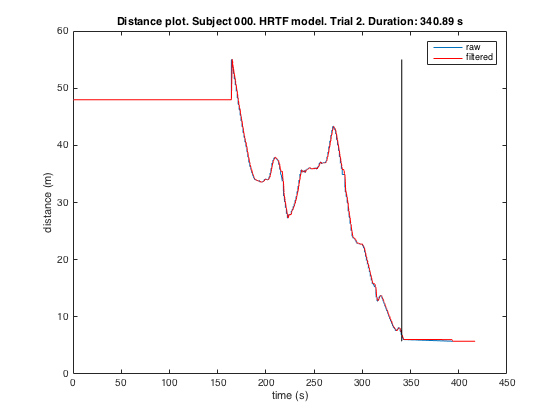
\includegraphics[scale=0.5]{graphics/subject000htrftrial2.png}
%  \caption{Distance plot of the subject number 000 using the HRTF model in the trial number 2, which had a duration of 340.89 seconds. Vertical line indicates the time when the subject found the sound.}
   \caption{Distance (related to the GPS sensor) remains constant the first 164 seconds. Vertical line indicates the time when the subject found the sound.}
  \label{fig:plt1}
\end{figure}

\setlength{\abovecaptionskip}{15pt plus 3pt minus 2pt} % Chosen fairly arbitrarily

\begin{figure}[h!]
  \centering
    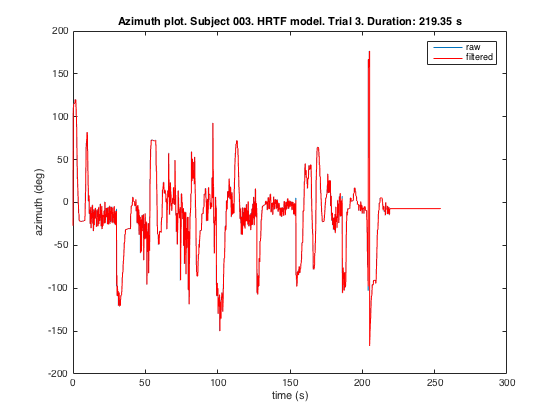
\includegraphics[scale=0.5]{graphics/subject003htrftrial3.png}
  \caption{Orientation is unreliable from 10 to 30 seconds}
  \label{fig:plt2}
\end{figure}

\setlength{\abovecaptionskip}{15pt plus 3pt minus 2pt} % Chosen fairly arbitrarily


\begin{figure}[h!]
  \centering
    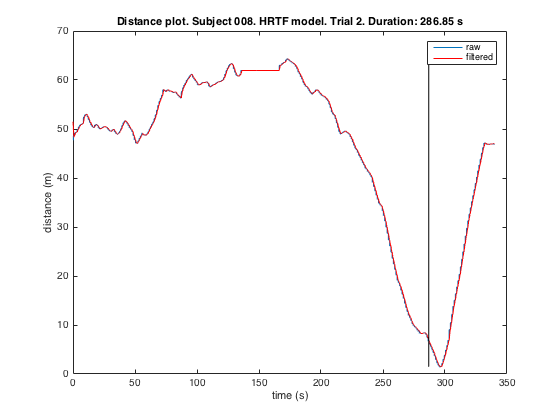
\includegraphics[scale=0.5]{graphics/subject008htrftrial2.png}
  \caption{Distance is constant for 30 seconds starting at mark 135 second}
  \label{fig:plt3}
\end{figure}

\setlength{\abovecaptionskip}{15pt plus 3pt minus 2pt} % Chosen fairly arbitrarily


\begin{figure}[h!]
  \centering
    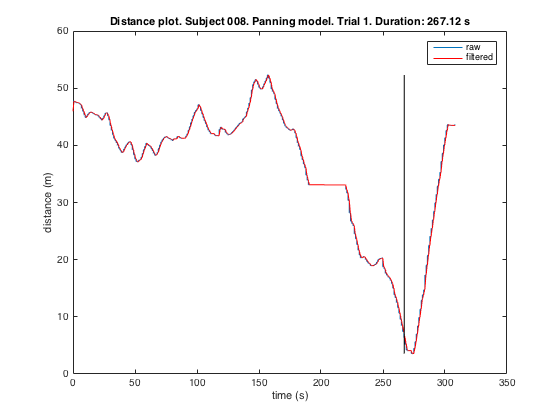
\includegraphics[scale=0.5]{graphics/subject008panningtrial1.png}
  \caption{Distance is constant for 30 seconds starting at mark 190 second}
  \label{fig:plt4}
\end{figure}

\begin{figure}[h!]
  \centering
    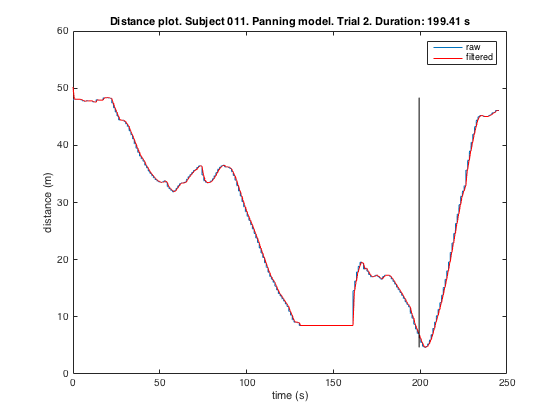
\includegraphics[scale=0.5]{graphics/subject011panningtrial2.png}
  \caption{Distance is constant for 30 seconds starting at mark 131 second}
  \label{fig:plt15}
\end{figure}

\begin{figure}[h!]
  \centering
    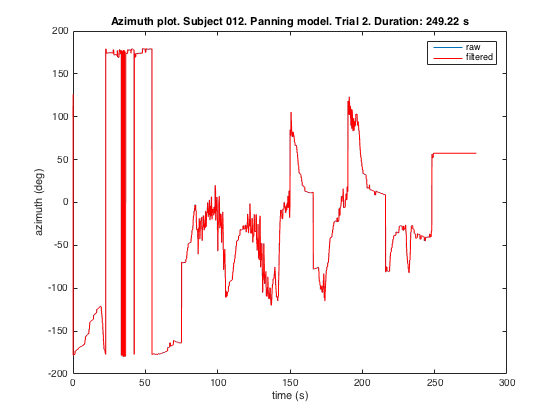
\includegraphics[scale=0.5]{graphics/subject012panningtrial2.png}
  \caption{Orientation is not reliable from 20 to 75 seconds}
  \label{fig:plt6}
\end{figure}

\section{Stimulus content}
``Hello, I am your test guide. If you can listen to my voice you are not far from me but you haven't found me yet. So, your task is to find where I am speaking as fast as you can. Please use your hearing and let you be guided through. Enjoy your search."

\section{Computing the azimuth}
\begin{algorithm}
\KwData{C++ pseudo-code to compute the azimuth:}
% computeAzimtuh(Geo::Coordinate soundGPScoord)\;
  new Latitude = myGPS Latitude - myGPS Latitude\;
  new Longitude = myGPS Longitude - myGPS Longitude\;
  newCoord = Geo::Coordinate(new Latitude, new Longitude)\;
  soundLat = soundGPS Latitude - myGPS Latitude\;
  soundLong = soundGPS Longitude - myGPS Longitude\;
  soundCoord = Geo::Coordinate(soundLat,soundLong)\;
  pointLat = new Latitude\;
  pointLong = abs(soundLat)\;
  pointCoord = Geo::Coordinate(pointLat,pointLong)\;
  adjacent = Geo::GeoUtils::distanceHaversine(pointCoord,soundCoord)\;
  opposite = Geo::GeoUtils::distanceHaversine(pointCoord,newCoord)\;
  hypo = Geo::GeoUtils::distanceHaversine(newCoord,soundCoord)\;
  gamma = asin(opposite/hypo)\;

  \If{the sound is in the first quadrant}
    {beta = 90 - gamma\;}
  \ElseIf{if the sound is in the fourth quadrant}
    {beta = 180 - gamma\;}
  \ElseIf{if the sound is in the third quadrant}
    {beta = 270 - gamma\;}
  \ElseIf{if the sound is in the second quadrant}
    {beta = 360 - gamma\;}

  \If{beta is bigger than 180}{
    \If{abs(beta - Angle to the North) is bigger than 180}{
      azimuth = abs(beta - Angle to the North) - 360\;}
    \Else{
      azimuth = beta - Angle to the North\;}
  \Else{
    \If{abs(beta - Angle to the North) is bigger than 180}{
      azimuth = abs(abs(beta - Angle to the North)) - 360\;}
    \Else{
    azimuth = beta - Angle to the North\;}
  }
  azimuth = round((azimuth * (PI / 180)))\;
  return azimuth\;
  }

\caption{algorithm that computes the azimuth}
\end{algorithm}

\section{Questionnaire answers}
In this section, the frequency for the responses of the questionnaire are included.
\begin{figure}[h!]
  \centering
    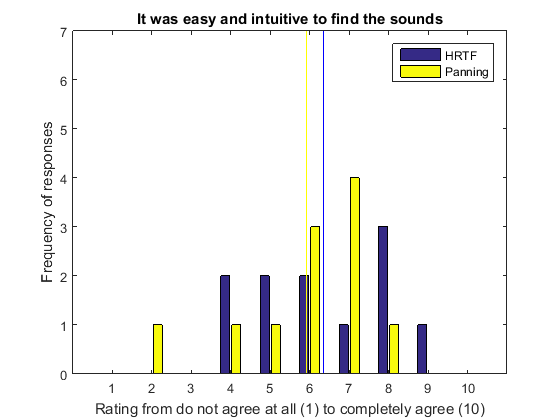
\includegraphics[scale=0.7]{graphics/qq1.png}
   \caption{Distribution of the answers for the questionnaire question "It was easy and intuitive to find the sounds"}
  \label{fig:plt1}
\end{figure}

\begin{figure}[h!]
  \centering
    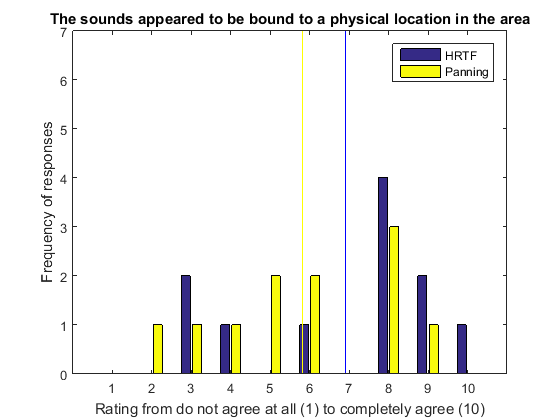
\includegraphics[scale=0.7]{graphics/qq2.png}
   \caption{Distribution of the answers for the questionnaire question "The sounds appeared to be bound to a physical location in the area"}
  \label{fig:plt1}
\end{figure}

\begin{figure}[h!]
  \centering
    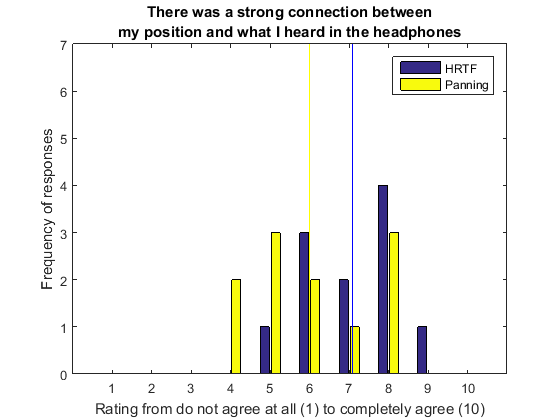
\includegraphics[scale=0.7]{graphics/qq3.png}
   \caption{Distribution of the answers for the questionnaire question "There was a strong connection between my position and what I heard in the headphones"}
  \label{fig:plt1}
\end{figure}

\begin{figure}[h!]
  \centering
    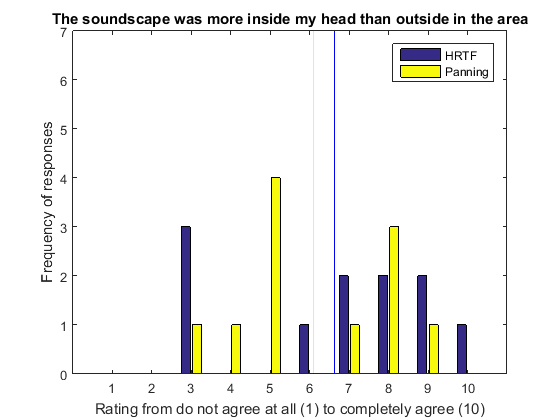
\includegraphics[scale=0.7]{graphics/qq4.png}
   \caption{Distribution of the answers for the questionnaire question "The soundscape was more inside my head than outside in the area"}
  \label{fig:plt1}
\end{figure}

\begin{figure}[h!]
  \centering
    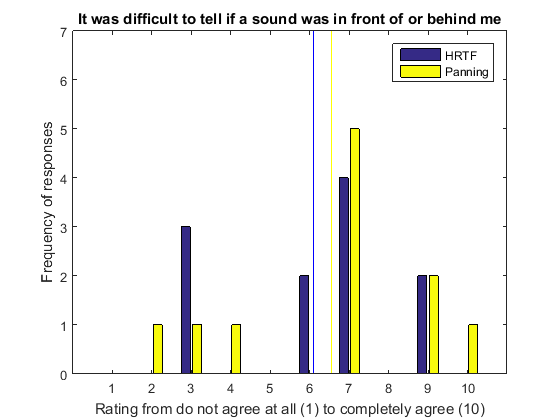
\includegraphics[scale=0.7]{graphics/qq5.png}
   \caption{Distribution of the answers for the questionnaire question "It was difficult to tell if a sound was in front of or behind me"}
  \label{fig:plt1}
\end{figure}


\end{appendices}
\pagebreak
% Style and bibliography.
% The bibtex filename
%bliography{}
% \section*{References}
\bibliographystyle{ieeetr}
\bibliography{biblio}

% that's all folks
\end{document}


